\chapter{Interactive Oracle Proofs and the BCS Transformation}
\label{ch:iop}

The FRI protocol of \cref{ch:fri} is an
\emph{interactive oracle proof} (IOP): the prover sends oracles that the
verifier queries at a few positions, rather than messages it reads in
full. This chapter introduces the IOP model and the BCS transformation
that compiles an IOP into a non-interactive argument by realising its
oracles as Merkle commitments and its queries as commitment openings.
Once this compiler is in place, the FRI protocol can be described purely
in terms of oracles and queries, leaving the commitment machinery
implicit.

\section{Merkle Trees}
\label{sec:merkle_trees}
% ==================================================================
A Merkle tree commits to a sequence of values by hashing them into a
tree. The whole sequence is represented by one value, the root, and any
position can later be revealed with a short proof. This is the device
that realises the oracles of an IOP.

\begin{definition}[Merkle Tree]
\label{def:merkle}
A \emph{Merkle tree} over a sequence $(v_0, v_1, \ldots, v_{N-1})$
is a complete binary tree where each leaf stores the hash of one
element, $\ell_i = H(v_i)$; each internal node stores the hash of the
concatenation of its two children,
$H(n_{\mathrm{left}} \| n_{\mathrm{right}})$; and the root $r$ is a
single digest that binds the entire sequence.
\end{definition}

The root has fixed length and depends on every element of the sequence.
Changing any $v_i$ changes its leaf hash $H(v_i)$, which changes every
node on the path from that leaf to the root, and so changes the root.
The root therefore \emph{binds} the sequence: this is made precise as
position binding in \cref{prop:position_binding} below, once openings
have been defined.



\subsection{Openings and the Authentication Path}
\label{subsec:merkle_opening}
 
To reveal the value at a position without sending the whole sequence,
the prover uses an authentication path. To open position $i$, it reveals
$v_i$ and the \emph{authentication path}: the sibling hashes along the
route from the leaf $\ell_i$ to the root, one per level, so $\log_2 N$
hashes in total.
 
With these siblings the verifier can recompute the root on its own, even
though it never sees the other leaves. It starts from $\ell_i = H(v_i)$
and, at each level, hashes the value it currently holds together with the
provided sibling, in the correct left-right order, obtaining the parent
node; repeating this up the tree yields a candidate root, which it
compares with the committed one. A single sibling per level suffices
because each node on the path is the hash of two inputs, the node and its
sibling; the sibling is the one input the verifier does not already hold.
The verifier accepts if the recomputed root equals the committed root.
The cost is $O(\log N)$ hash evaluations.
 
\Cref{alg:rootfrompath} makes this recomputation explicit. The order in
which each sibling is combined, whether the current node goes on the left
or on the right, is dictated by the bits of the position $i$: at level
$\ell$, the $\ell$-th bit of $i$ (counting from the leaf) is $0$ when the
current node is a left child, so the sibling is hashed on its right, and
$1$ when it is a right child, so the sibling goes on its left.
 
\begin{algorithm}
\caption{$\mathsf{RootFromPath}$: recompute the root from an opening.}
\label{alg:rootfrompath}
\begin{algorithmic}[1]
\Require value $v_i$, position $i$, sibling hashes $(s_1, \ldots, s_d)$
\State $\mathit{node} \gets H(v_i)$ \Comment{start from the leaf}
\For{$\ell = 1$ \textbf{to} $d$}
  \If{$\mathrm{bit}_\ell(i) = 0$}
    \State $\mathit{node} \gets H(\mathit{node} \,\Vert\, s_\ell)$
      \Comment{current node is a left child}
  \Else
    \State $\mathit{node} \gets H(s_\ell \,\Vert\, \mathit{node})$
      \Comment{current node is a right child}
  \EndIf
\EndFor
\State \Return $\mathit{node}$ \Comment{accept iff equal to the committed root}
\end{algorithmic}
\end{algorithm}
 
\begin{example}
\label{ex:merkle}
For four values $(v_0, v_1, v_2, v_3)$ the tree has leaves
$\ell_i = H(v_i)$, two internal nodes $H(\ell_0 \Vert \ell_1)$ and
$H(\ell_2 \Vert \ell_3)$, and a root hashing the two. To open position
$2$, the prover reveals $v_2$ and the two siblings $s_1 = \ell_3$ and
$s_2 = H(\ell_0 \Vert \ell_1)$; here the depth is $d = 2$ and the position
in binary is $i = 2 = (10)_2$.
 
Running \cref{alg:rootfrompath} on this input:
\begin{itemize}
  \item start: $\mathit{node} = H(v_2) = \ell_2$;
  \item level $1$: $\mathrm{bit}_1(2) = 0$, so $\ell_2$ is a left child
    and $\mathit{node} \gets H(\ell_2 \Vert s_1) = H(\ell_2 \Vert \ell_3)$;
  \item level $2$: $\mathrm{bit}_2(2) = 1$, so the current node is a right
    child and
    $\mathit{node} \gets H(s_2 \Vert \mathit{node})
      = H\bigl(H(\ell_0 \Vert \ell_1) \Vert H(\ell_2 \Vert \ell_3)\bigr)$.
\end{itemize}
The final value is the root, which the verifier compares with the
committed one (\cref{fig:merkle}). The two revealed siblings were exactly
what was missing at each level to move one step up.
\end{example}
 
\begin{figure}[ht]
\centering
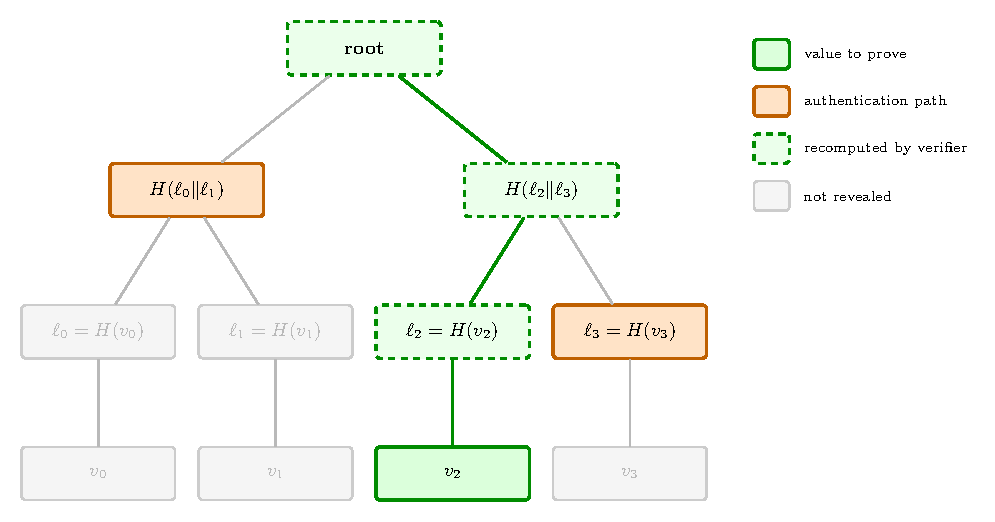
\includegraphics[width=0.9\textwidth]{images/merkle_tree.pdf}
\caption{Verification of $v_2$ in a four-leaf Merkle tree. The prover
reveals the \emph{authentication path} (the two siblings $\ell_3$ and
$H(\ell_0\Vert\ell_1)$, in orange); the verifier recomputes the dashed
nodes from $v_2$ up to the root and compares the result with the
committed root. The greyed-out nodes are never revealed.}
\label{fig:merkle}
\end{figure}


\subsection{A Vector Commitment}
\label{subsec:merkle_vc}
 
A Merkle tree is a \emph{vector commitment}. The prover commits to a
vector with the root, and later opens any position with an authentication
path. Its security property is \emph{position binding}: after publishing
a root, the prover cannot open one position to two different values.
 
\begin{proposition}[Position Binding]
\label{prop:position_binding}
Let $H$ be a random oracle. No efficient prover can output a root
$r$, a position $i$, a length $N$, and two openings $(v, p)$ and
$(v', p')$ for position $i$ with $v \neq v'$ such that both recompute to
$r$, except with negligible probability.
\end{proposition}
 
By position binding, a Merkle root can stand in for an oracle. The
committed vector is fixed, and the prover cannot change the value at a
queried position after committing.

% ==================================================================


\section{Interactive Oracle Proofs}
\label{sec:iop}
% ==================================================================


An interactive oracle proof generalises the interactive proofs of
\cref{subsec:interactive_proofs}. As there, prover and verifier exchange
messages over several rounds; the new element is that the verifier does
not read the prover's messages in full, but is given \emph{oracle access}
to them, querying only a few chosen positions.

% BCS16, Definition 2.2.
\begin{definition}[Interactive Oracle Proof
  {\cite[Definition~2.2]{BCS16}}]
\label{def:iop}
An \emph{Interactive Oracle Proof} (IOP) for a language $\mathcal{L}$
is an interactive protocol between a prover $\Prover$ and a verifier
$\Verifier$ that proceeds in rounds. In each round:
\begin{enumerate}
  \item the prover sends an \emph{oracle message} $\pi_i$ (a function
    that the verifier may query at chosen positions);
  \item the verifier sends a random challenge $r_i$.
\end{enumerate}
After $k$ rounds, the verifier makes a bounded number of queries to
$\pi_1, \ldots, \pi_k$ and outputs $\mathsf{accept}$ or
$\mathsf{reject}$.
\end{definition}

\begin{example}
\label{ex:iop}
FRI is itself an IOP. In each round the prover's oracle is a codeword,
and the verifier's challenge is a folding coefficient; at the end the
verifier queries only a handful of positions of each oracle rather than
reading the full codewords, which is what makes verification succinct.
The oracles are treated abstractly here; their concrete realisation as
Merkle commitments is deferred to the BCS transformation.
\end{example}

The key difference from a standard interactive proof is that the
verifier has \emph{oracle access} to the prover's messages: rather than
receiving each message in full, it may query a small number of chosen
positions of $\pi_i$. The oracle is an abstraction: it fixes the
message in advance, so that every query is answered consistently, but
says nothing about how this is realised. Making the oracles concrete is
the job of the BCS transformation of \cref{sec:bcs}, after which we can
reason about FRI purely in terms of oracles and queries, without
committing to any particular implementation of them.

An IOP of \emph{proximity} (IOPP) is an IOP in which the verifier tests
whether the prover's initial oracle is close to a codeword of a
specified code, rather than testing membership in a
language~\cite{BBHR18}. FRI, described in \cref{ch:fri}, is an IOPP for
Reed-Solomon codes.


 
% ==================================================================
\section{The BCS Transformation}
\label{sec:bcs}
% ==================================================================
 
The IOP model of \cref{sec:iop} leaves two things abstract: the oracle
messages, which the verifier can query but not read in full, and the
interaction, which requires the verifier to send live random challenges.
The BCS transformation~\cite{BCS16} removes both, compiling an IOP into a
non-interactive argument in the random oracle model. It does so by
realising each abstract ingredient with a concrete one.
 
\begin{itemize}
  \item \textbf{Oracles become commitments.} Each oracle message
    $\pi_i$ is replaced by a Merkle commitment to its values
    (\cref{sec:merkle_trees}): the prover builds a Merkle tree over
    $\pi_i$ and sends only the root. By position binding, the root fixes
    the message so that it cannot be changed after the fact, which is the
    role the oracle played in the IOP. This is where the Merkle trees
    commit to the oracle messages: in FRI the prover evaluates a
    polynomial on the FRI domain, builds a Merkle tree over the
    evaluations, and sends the root to the verifier.
  \item \textbf{Queries become openings.} When the verifier queries
    position $j$ of $\pi_i$, the prover answers with the value together
    with its authentication path, and the verifier checks the path
    against the committed root. An opening that verifies is a consistent
    answer to an oracle query.
  \item \textbf{Challenges become random-oracle outputs.} Each verifier
    challenge is set to the output of the random oracle on the transcript
    so far (\cref{subsec:fiat_shamir}), so no live interaction is needed
    and the whole exchange becomes a single message. The challenge of a
    round is fixed only after the commitment of that round is in the
    transcript, which preserves soundness.
\end{itemize}
 
Carried out on a round-by-round sound IOP, the two steps give the
sequence
%
\[
\text{IOP}
\;\xrightarrow{\ \text{BCS}\ }\;
\text{interactive argument}
\;\xrightarrow{\ \text{Fiat-Shamir}\ }\;
\text{non-interactive argument} ,
\]
%
all in the random oracle model, where the soundness error of the final
argument is that of the IOP together with the binding error of the Merkle
commitments.
 
Because of this compiler, once an IOP is specified we may describe it at
the level of oracles and queries: it is enough to say that the prover
sends the oracle for a claimed codeword and that the verifier queries it
at chosen positions, with the understanding that the oracles are Merkle
commitments and the queries their openings. We adopt this style in
\cref{ch:fri}, where the resulting FRI IOP is compiled into a
non-interactive argument through the transformation described here.
 